\documentclass{standalone}

\usepackage{times}
\usepackage{amsmath}
\usepackage{amssymb}

\usepackage[dvipsnames]{xcolor}
\usepackage{tikz}
\usetikzlibrary{arrows,backgrounds,scopes}

\usepackage{pgfplots}
\pgfplotsset{compat=1.15}

%ICPC logo colors
\definecolor{red}{HTML}{972e21}
\definecolor{yellow}{HTML}{ebb83f}
\definecolor{blue}{HTML}{5e7fbf}
\definecolor{green}{HTML}{5fd94e}

\begin{document}
	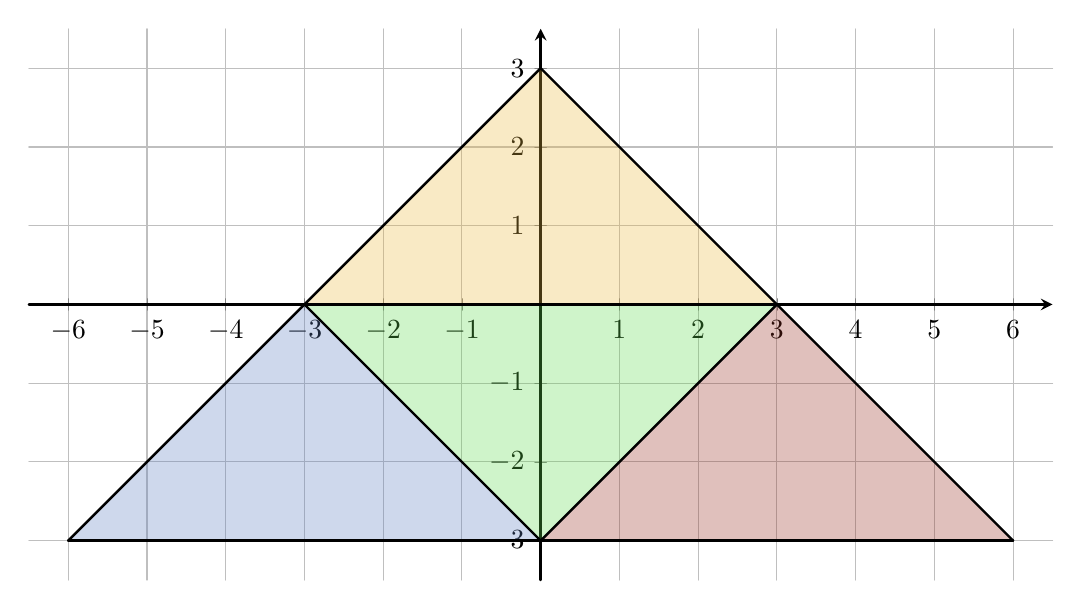
\begin{tikzpicture}[every path/.style={line cap=round, line width=0.03cm}]
		
		\begin{axis}[
			x=1.0cm,y=1.0cm,
			axis lines=middle,
			ymajorgrids=true,
			xmajorgrids=true,
			xmin=-6.5,
			xmax=6.5,
			ymin=-3.5,
			ymax=3.5,
			xtick={-6,-5,...,6},
			ytick={-3,-2,...,3},]
			
			\fill[blue,opacity=0.3] (-3,0) -- (0,-3) -- (-6,-3) -- cycle;
			\fill[yellow,opacity=0.3] (-3,-0) -- (3,0) -- (0,3) -- cycle;
			\fill[red,opacity=0.3] (3,0) -- (6,-3) -- (0,-3) -- cycle;
			\fill[green,opacity=0.3] (-3,0) -- (3,0) -- (0,-3) -- cycle;
			
			\draw (-6,-3) -- (0,3);
			\draw (0,3) -- (6,-3);
			\draw (6,-3) -- (-6,-3);
			\draw (-3,0) -- (3,0);
			\draw (3,0) -- (0,-3);
			\draw (0,-3) -- (-3,0);		
		\end{axis}
	\end{tikzpicture}
\end{document} 
